\documentclass[14pt letter paper]{article}
\usepackage[utf8]{inputenc}
\usepackage{graphicx}
\graphicspath{ {C:\Users\Gopi\Desktop\socialnetwork.jpg} }

\title{Sample Latex Assignment}
\author{Gopichandu.Para} 
        
\date{ 05 Feb 2016}


\begin{document}
\maketitle "De-anonymization Attack" \\A practical attack to De-Anonymize social networking users





\section{Introduction}
In the present generation and in the present Internet world every one gets used to social networking sites such as face book , twitter, linked-in, outlook, etc... \\According to the information provided by the social networking sites , the growth rate is getting increased year by year. As of now we have millions of users for face book, twitter and other social networking sites.
\\As we know that "Where there is a will there is a way".This is a good statement when we use it for good and in the same way it is a bad statement if we use it for doing something wrong. So in that sense as users in the networking sites are getting increased, the problems are getting increased. 


\begin{figure}[h]
\centering
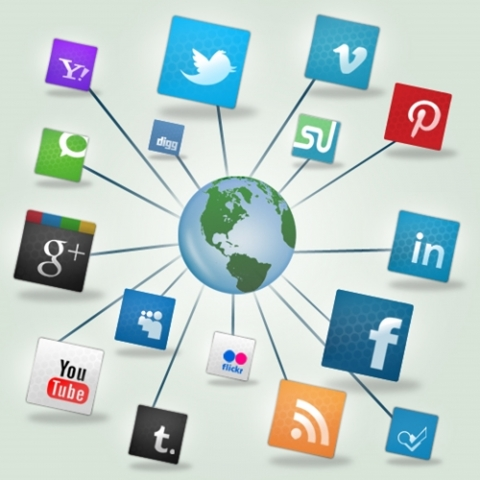
\includegraphics[width=9cm, height=6cm]{socialnetwork.jpg}
\caption{Social Networking Sites}
\label{fig:socialnetwork}
\end{figure}

There are some countries which blocked just "face book and not all the social networking sites. The countries which blocked Face book are shown in the table below. 

\begin{table}
 \begin{tabular}{||c c c c c c c||} 
 \hline
 Country & Face book & Google+ & You tube & Twitter & Linked-in & Instagram \\ [7ex] 
 \hline
 Egypt & NA & A & A & A & A & A \\ 
 \hline
 China & NA & A & A & A & A & A \\
 \hline
 Pakistan & NA & A & A & A & A & A \\
 \hline
 Syria & NA & A & A & A & A & A  \\
 \hline
 Bangladesh & NA & A & A & A & A & A \\
 \hline
 North Korea & NA & A & A & A & A & A \\
 \hline
 Vietnam & NA & A & A & A & A & A \\
 \hline
 Cuba & NA & A & A & A & A & A \\
 \hline
 Mauritius & NA & A & A & A & A & A \\ 
 \hline
 Iran & NA & A & A & A & A & A \\ [5ex] 
 \hline
\end{tabular}
\caption{Table shows countries which banned face book}   NA- Not Available \hspace{2cm} A-  Available
\label{table:1}
\end{table}

\section{About}
So, as shown in the figure above all the social networking sites are globally connected. Attacking is the main problem in the globally connected networks. So in this case using the "de-Anonymizing attack" we can simply identify the group or the team members who are connected in the network instead of tracking the browser cookies. "De-anonymization attack" helps a lot in this case.When the social networking users enters into a malicious website our de-anonymizing attack can easily identify them. 
 \\ This attack requires low effort and we can gain as much as information as possible from the user. This attack mainly performs theoretical analysis and logical measurements to demonstrate or define the capability of the attack against "Xing". Xing has a total of nearly eight million users in its account. This type of social networking site is mainly used for developing business relationships.

 \section{Group Member Enumeration}
 How can the attacker gets information about group members?
 \\Generally the social networks offer Public groups in which users can find useful information and join the group in which they find some known people. The attacker can collect the group information by simply joining into the group from directory, list all members and leave the group. May be after some time or on the spot it self the attacker can know the information of member of the group.
 
 \section{Action of reducing severity:}
 Reducing severity distinguishes between server side, client side, browser side.
 \\(a) Client side: \\ On the client side we can disable the browsing history and to open in the safe browsing mode.
 \\ (b)Browsing side: \\ Prevent access to style information links. what ever the browsers that updates after 10 years from now will fix history stealing.
 \\ (c) Server side: \\ Blocking the HTTP GET parameters with sensitive parameters. Adding tokens to sensitive URL's
 \\According to Incognito-Like Algorithm the total running time of performing these attacks is 

 \begin{equation}
O((p^2n_s + pn^3_s l)R).
\end{equation}
\\ According to Mondrian-like algorithm the total running time is 

\begin{equation}
O((p^2n_s + pn^3_s l)R).
\end{equation}

\section{Summary} Social networks are used to collect data with ID which is a group feature to identify victims quickly. In order to save the details every website can activate the de-anonymization code to find user profiles and trace the group with history stealing. In this attack we can find the different anonymity techniques. Effort for including and performing the attack is relatively low by using the de-anonymization.
\end{document}
\end{document}
 



